% TeX root=../main.tex

Karkamiš foi a principal cidade-estado neo-hitita na idade do ferro.
As fontes assírias com frequência confundem \emph{Hatti} e \emph{Karkamiš},
indicando que, ao menos do ponto de vista da política externa, a cidade era tida
como a herdeira do legado geopolítico do reinado hitita após sua queda.
Os hititas controlavam a região desde pelo menos \emph{circa} 1340 \textsc{aec},
quando Suppiluliuma I instala seu filho, Piyassilis, no trono de Karkamiš, sob o
nome Šarri-Kušuh.\footnote{A região parece ter sido ocupada desde \emph{circa}
	2400 \textsc{aec}.}
A dinastia de Šarri-Kušuh parece ter mantido o controle da região por diversas
gerações, atravessando a queda do reinado hitita em \emph{circa} 1190
\textsc{aec} e seus descendentes frequentemente reivindicaram a associação com
Suppiluliuma.

O sítio arqueológico foi associado com a cidade bíblica de Carquemis (hebr.\
\foreignlanguage{hebrew}{כַּרְכְּמִישׁ}) por George Smith em 1876, embora já fosse
conhecido de anos anteriores como fonte de esculturas e inscrições variadas.
As escavações realizadas pelo British Museum começam em 1878--81, são
interrompidas pela primeira guerra mundial e reiniciadas em 1920,
simultaneamente com o estabelecimento da fronteira sírio-turca como resultado da
partição dos territórios controlados pelos britânicos e franceses estabelecida
no acordo de Sykes-Picot.
A fronteira separou as cidades de Cerablus (Turquia, renomeada para Karkamış em
1946) e Jerabulus (Síria), dividindo o sítio arqueológico em duas partes, o
que causou interrupções frequentes nas escavações.
Embora ocupado pelo menos desde o segundo milênio \textsc{aec}, a maior parte
das descobertas arqueológicas representam o estado do assentamento durante
a idade do ferro.




\begin{center}
	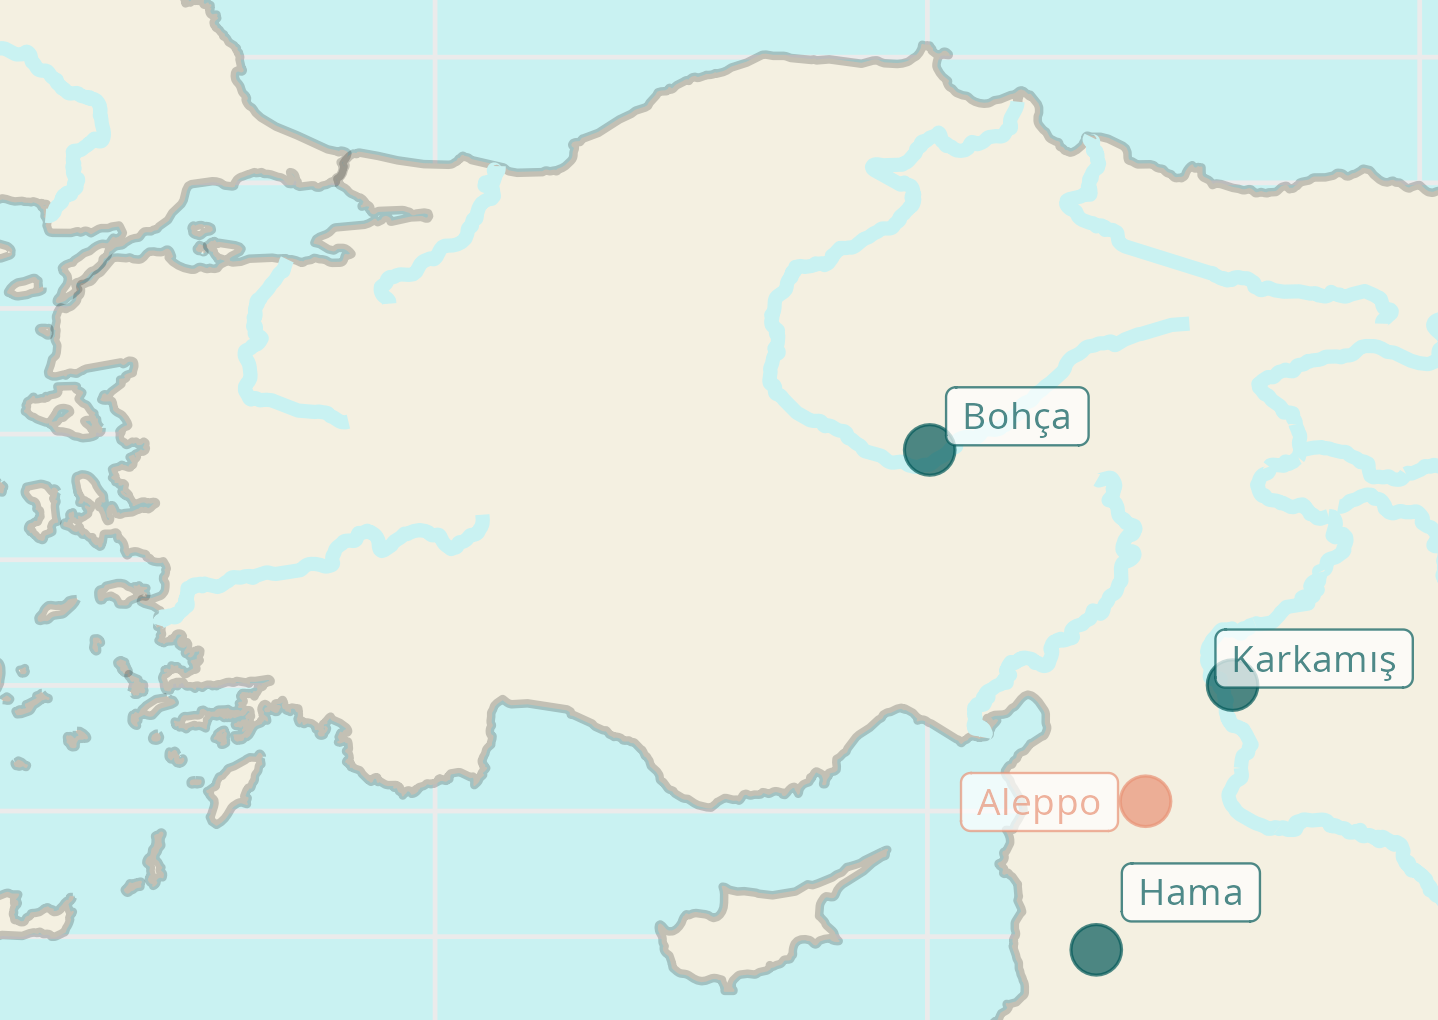
\includegraphics[width=0.8\textwidth]{../../../Mídia/Map04.png}
\end{center}

\clearpage

Karkamiš teria sido uma cidade fortificada por duas camadas de muralhas, o
centro administrativo estando na esfera mais interna, com acesso direto ao rio
Eufrates ao nordeste.
Dentro deste círculo, entende-se que a cidade teria dois complexos palaciais, um
na cidade baixa e o outro na cidade alta.
A parte mais bem escavada é o complexo palaciano inferior, com
construções identificadas desde o portão ao lado do rio Eufrates até o portão
real que levaria à cidade alta.

\begin{figure}[h!]
	\begin{center}
		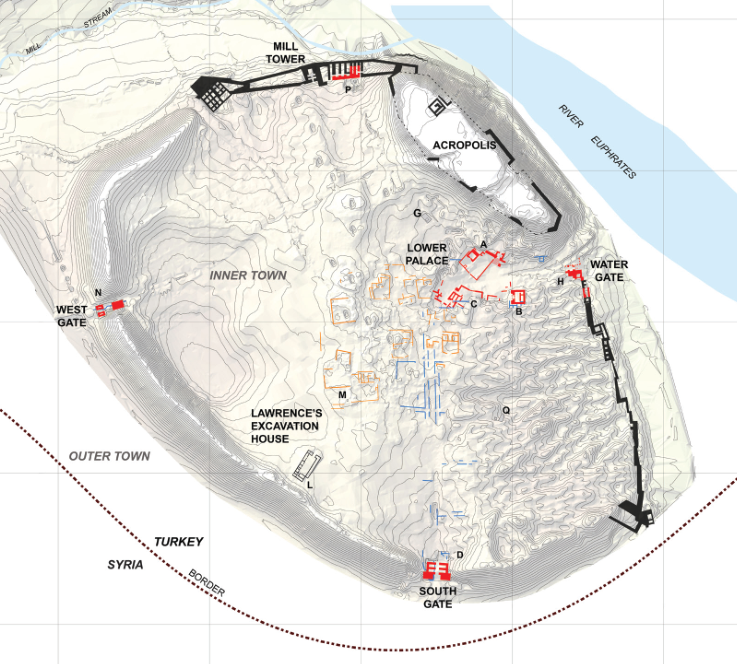
\includegraphics[width=0.8\textwidth]{../../../Mídia/karkemis00.png}
	\end{center}
	\begin{center}
		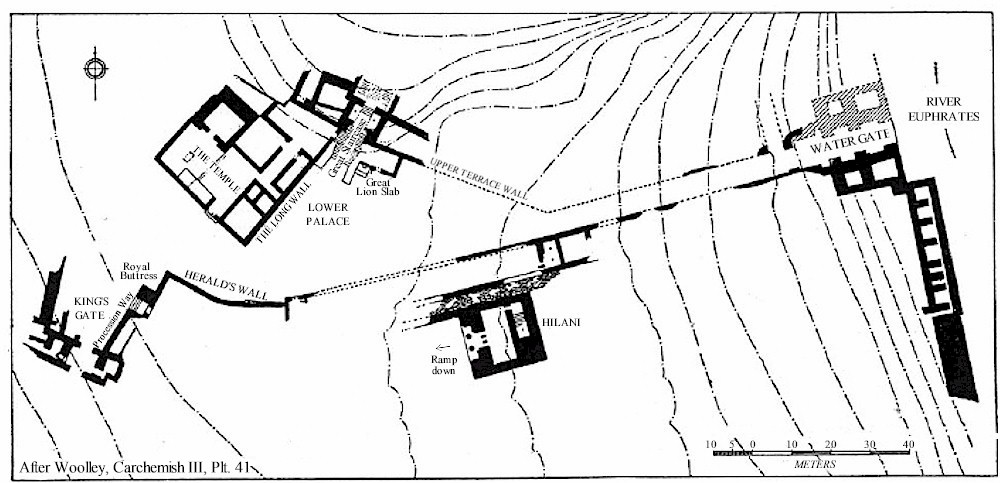
\includegraphics[width=\textwidth]{../../../Mídia/kargamis01.jpg}
	\end{center}
	\caption[Mapas de Karkamiš]{Mapas de Karkamiš~\cite[22]{Marchetti2014} e do
		complexo palaciano inferior~\cite[\emph{plate} 41]{CarchemishIII}.}\label{fig:mapa-kark1}
\end{figure}

A maior parte das inscrições provém de ortostatos (blocos de pedra verticais
utilizados na construção de um muro), incluindo KARKAMIŠ A11\emph{b}+\emph{c} (=
A9 e 10).
Escavados nas operações de 1911--14, as peças tinham sido reutilizadas como
pavimento, com o texto virado para baixo,
no umbral do ``Portão do Rei'', próximas da inscrição A11\emph{a},
encontrada \emph{in situ} (\autoref{fig:portao-real}).

\begin{figure}[h!]
	\begin{center}
		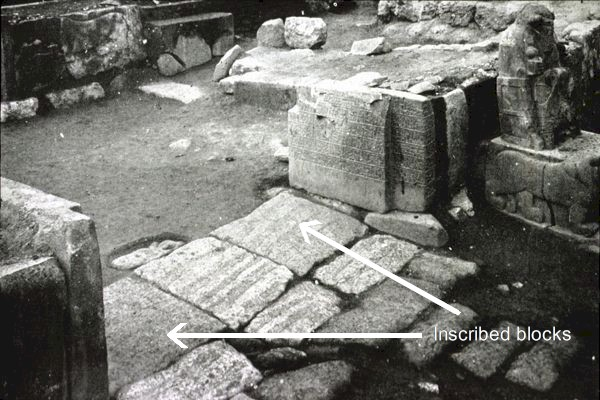
\includegraphics[width=0.95\textwidth]{../../../Mídia/kargamis08.jpg}
		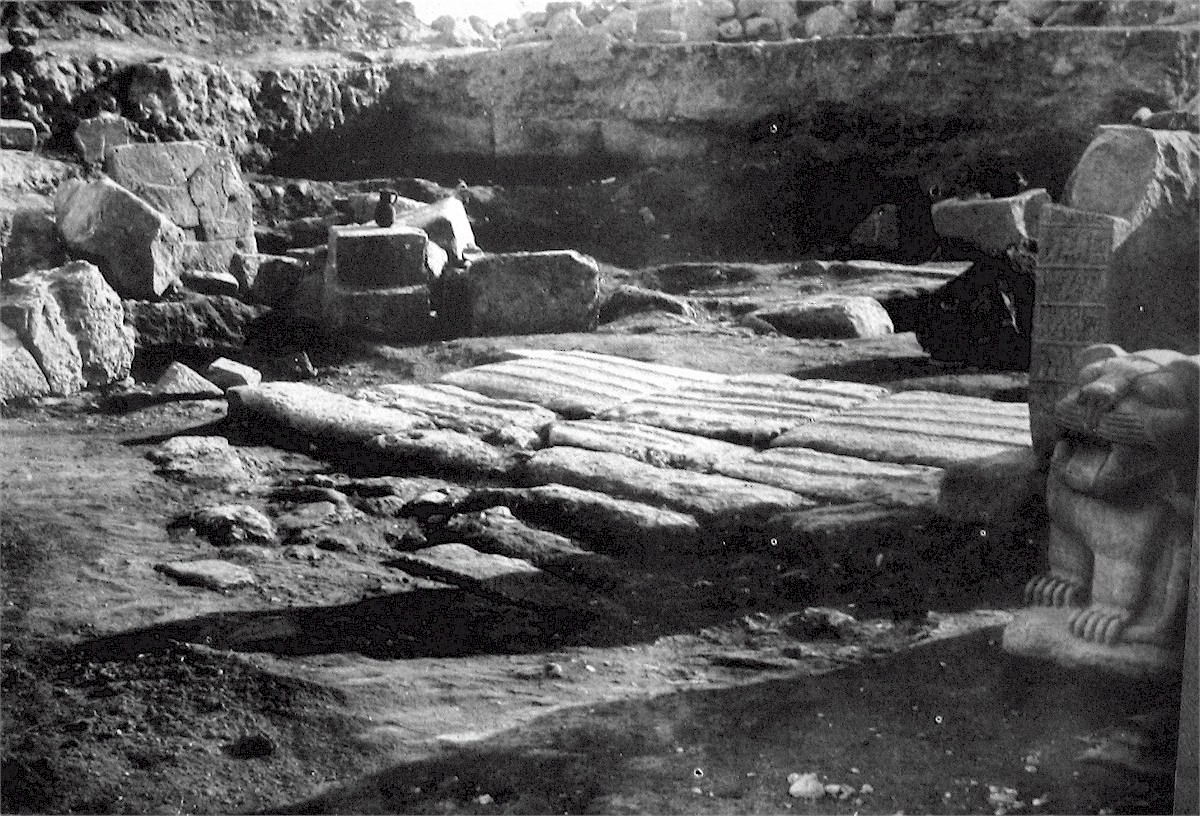
\includegraphics[width=0.95\textwidth]{../../../Mídia/kargamis111.jpg}
	\end{center}
	\caption[``Portão do Rei'' em Karkamiš]{Portão do Rei em Karkamiš. Em pé
		vê-se a inscrição A11\emph{a} e o pavimento imediatamente ao lado é
		composto pelos ortostatos da inscrição A11\emph{b}+\emph{c}. Imagens
		de~\cite[\emph{plates} 46--7]{CarchemishIII}.}\label{fig:portao-real}
\end{figure}



O conteúdo do texto de KARKAMIŠ A11\emph{b}+\emph{c} e o material utilizado
fazem supor que os dois ortostatos utilizados na inscrição faziam parte do
``Contraforte Real'', antes do ``Caminho de Procissão'', alguns metros antes do
``Portão do Rei'' (ver~\autoref{fig:mapa-kark1}) e
as peça A11\emph{b} (= A9) e A11\emph{c} (= A10) devem ter sido parte de batentes
de uma porta \slash{} portão, dispostas do lado direito e esquerdo,
respectivamente.
As peças narram o que parece ter sido uma revolta na cidade protagonizada por
figuras mencionadas por \emph{netos de Uratarhunta}; a reconquista da cidade
simultaneamente à conquista de Kawa com apoio dos deuses; a construção dos
andares superiores do ``Caminho de Procissão'' e o estabelecimento de culto às
divindades Tarhunta, Karhuha, Kubaba e Sarku.
Em meio ao texto, estabelece-se os sacrifícios estipulados às divindades,
maldições de proteção e uma justificativa para a construção dos andares
superiores, talvez indicando que o uso deste espaço seria voltado a mulheres de
alguma forma.
Os ortostatos hoje estão no Anadolu Medeniyetleri Müzesi em Ankara.

\begin{figure}[h]
	\centering
	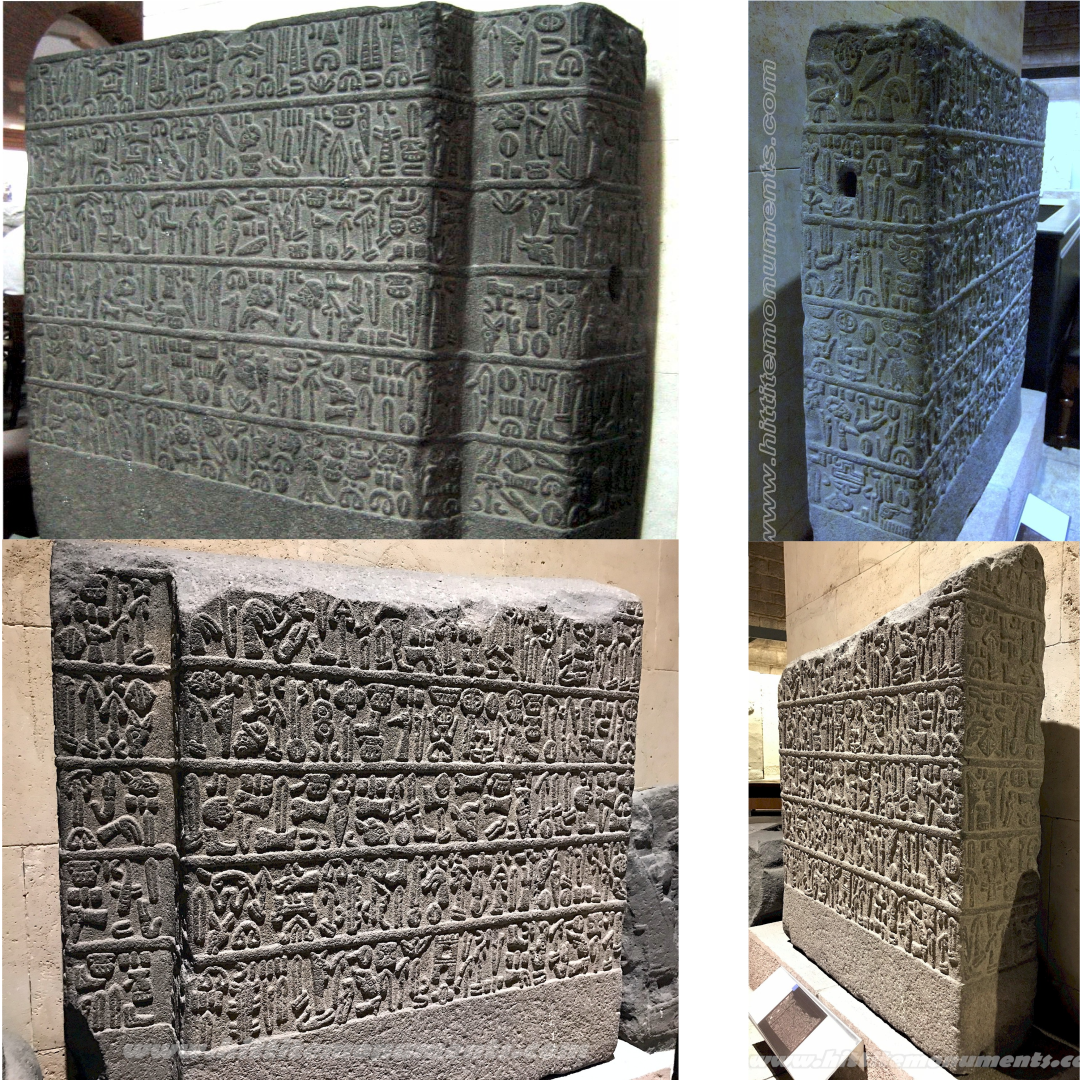
\includegraphics[width=0.9\textwidth]{../../../Mídia/karkamisA11bc.png}

	\caption[KARKAMIŠ A11\emph{b}+\emph{c}]{Inscrição KARKAMIŠ A11\emph{b}+\emph{c}.
		Dimensões da inscrição:
		\emph{b} 0.83\times1.60\times0.23m,
		\emph{c} 0.86\times1.55\times0.23m.
		Imagens de Tayfun Bilgin, 2006,
		disponíveis em
		\href{https://www.hittitemonuments.com/karkamis/kargamis43.htm}{Hittite Monuments}.
		Edição e traçado em~\citeabbrev*{CHLI11}, pp.\ 101ff.\ e \emph{plate}
		14--17.
	}\label{fig:karkamisA11b}
\end{figure}

\begin{center}
	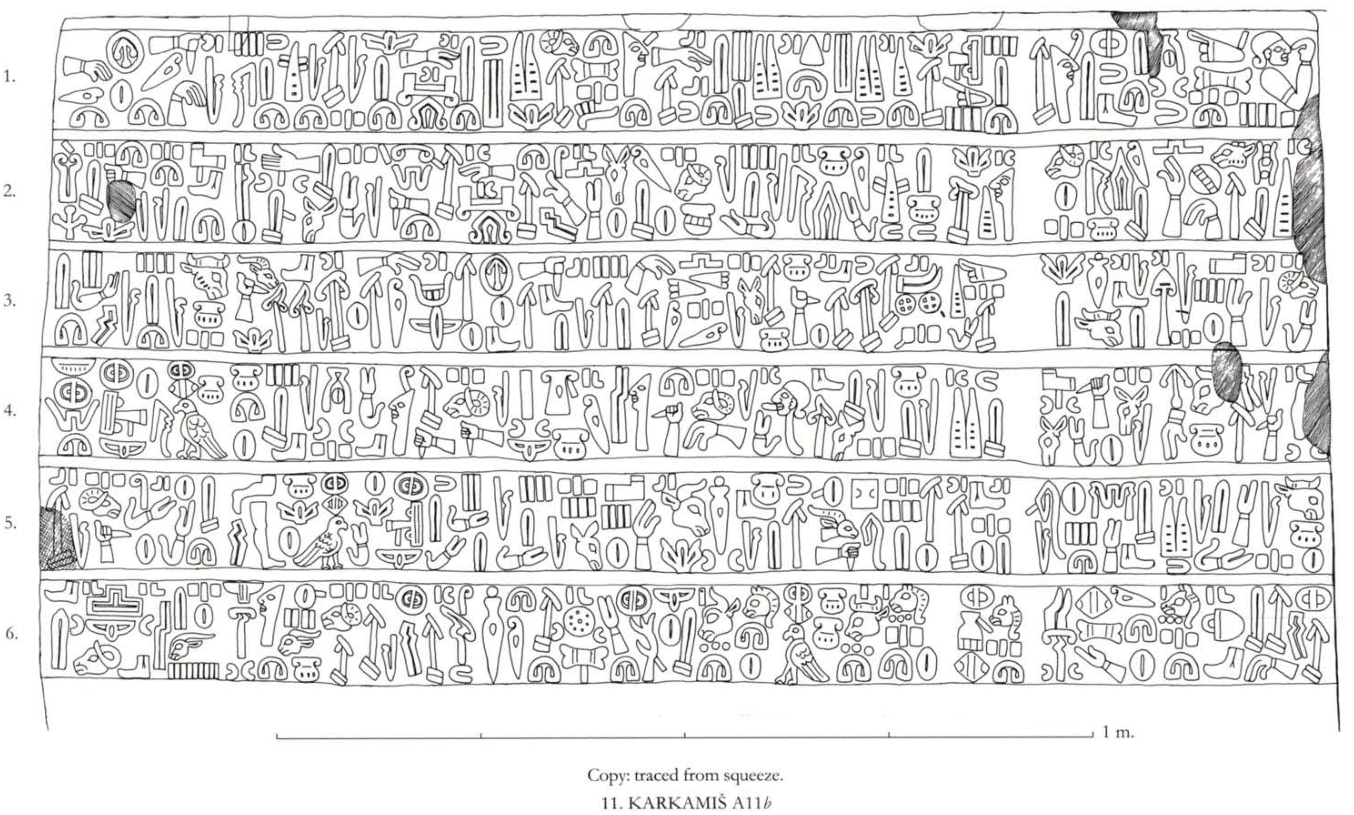
\includegraphics[height=\textwidth, angle=90]{../../../Mídia/karkamisA11b.png}
\end{center}

\clearpage

\begin{center}
	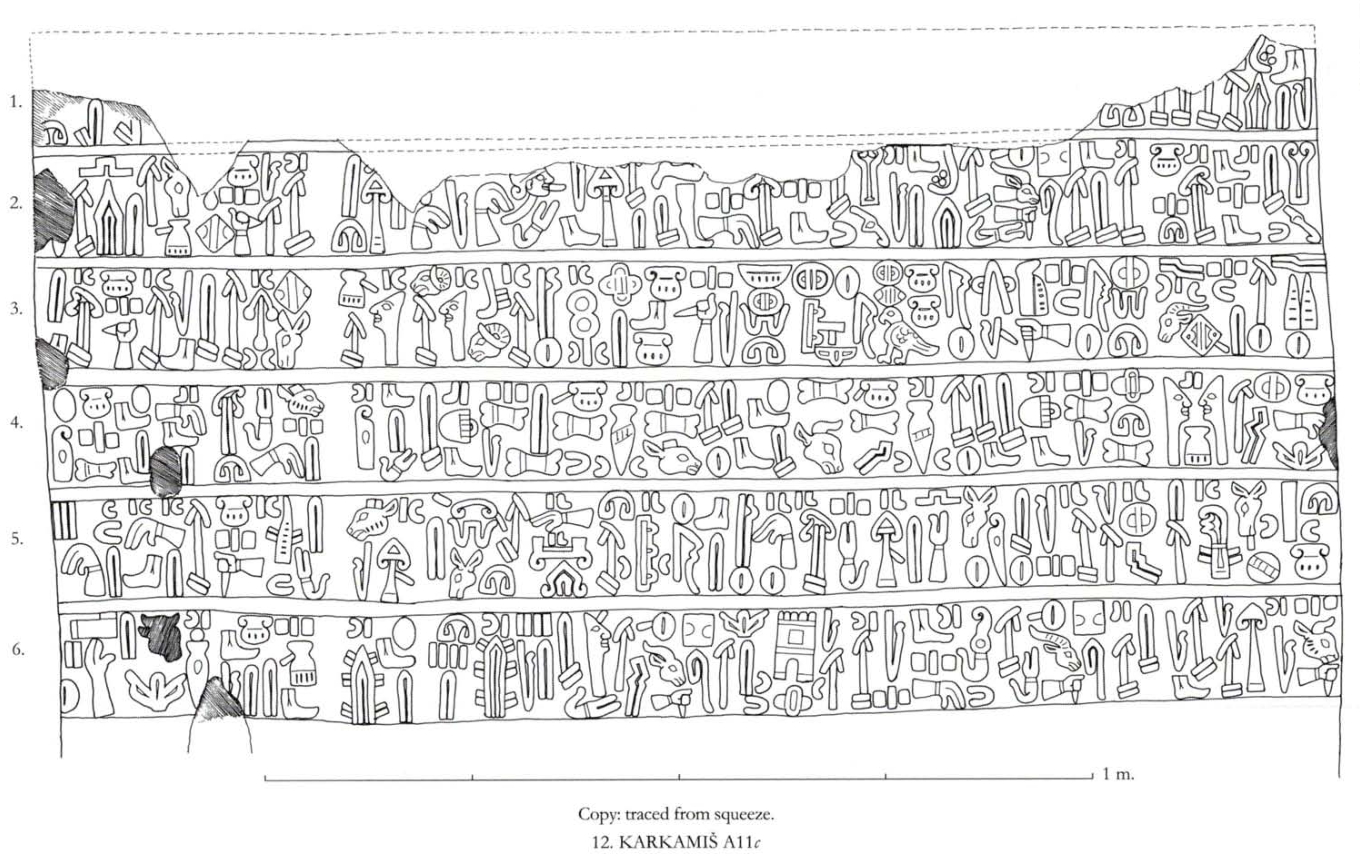
\includegraphics[height=\textwidth, angle=90]{../../../Mídia/karkamisA11c.png}
\end{center}

\clearpage

\setcounter{parcount}{0}
\begin{parnumbersa}[]

	\raggedright%
	\itshape%

	\logo{EGO}-wa/i-mi \spac{}ka-tú-wa/i-sa \logo{“IUSTITIA”}-ni-i-sa
	\logo{DEUS}-ni-ti-i \logo{(LITUUS)}á-za-mi-i-sa
	kar-ka-mi-si-za-sa\logo{(URBS)} \lmasc{}\logo{REGIO}-ni \logo{DOMINUS}-sa
	\spac{}su-hi-si \lmasc{}\logo{REGIO}-ni \logo{DOMINUS}-ia-i-sa
	\lmasc{}\logo{FILIUS.}NI-za-sa \spac{}á-sa-tú-wa/i-lá/í-ma-za-si \logo{REGIO}-ni \logo{DOMINUS}-i-sa \lmasc{}\logo{FILIUS.NEPOS}-si-i-sa

	a-wa/i za-a-sa \logo{URBS+}MI-ni-i-sa mi-sá-*a \lmasc{}tá-da-li-sa
	\logo{AVUS}-ha-da-li-sa \lbreak{} \spac{}\logo{*447}-nu-wa/i-ia-si sa-tá-*a

	wa/i-sa-*a \logo{VACUUS}-ti-i-sa \lmasc{}\logo{ARHA} \logo{(“LONGUS”)}ia\logo{+} ra/i-ia-ta

	wa/i-na-*a \spac{}\logo{MAGNUS+}ra/i-\logo{TONITRUS}-tá-sa-za \lmasc{}\logo{FILIUS.NEPOS}-sa-za \logo{CUM}-ní \lmasc{}\logo{(LOCUS)}pi-ta-ha-li-ia-ha

	wa/i-ma-zá-*a mi-i-na-*a \lmasc{}sá-pa-la/i-li-na \lmasc{}\logo{URBS+}MI-ni i-pa-ni-si-ná\logo{(URBS)} \lmasc{}á-ma-ha-wa/i \lmasc{}sá-pa-lá/í-li-ia \logo{TERRA.PONERE}-ru-da mu-zi-ki-ia\logo{(URBS)} \lmasc{}$[$\logo{\ldots{}}$]$ \lbreak{}

	wa/i-ma-na-a* \lmasc{}\logo{AEDIFICARE}-\logo{MI}-ha

	a-wa/i \lmasc{}\logo{REL}-a-ti-i \lmasc{}\logo{(ANNUS)}u-si-i
	ka-wa/i-za-na\logo{(URBS)} \lmasc{}\logo{(CURRUS)}wa/i\logo{+}ra/i-za-ni-ná
	\lmasc{}\logo{PES\textsubscript{2}}-za-ha

	pa-tá-za-pa-wa/i-ta-*a \logo{(TERRA+LA+LA)}wa/i-li-li-da-za mi-i-zi-*a
	\lmasc{}tá-ti-i-zi \logo{AVUS}-ha-ti-zi-ha
	\lmasc{}\logo{*348}{(-)}lu/a/i\textsuperscript{?}-da-li-zi-ha
	\lmasc{}\logo{NEG\textsubscript{2}}-a \logo{(PES\textsubscript{2})}hwi/a-hwi/a-sà-tá-si


\end{parnumbersa}

\vspace{10pt}
\hrule
\vspace{10pt}


\setcounter{parcount}{0}
\begin{parnumbersa}[]

	\raggedright%
	\itshape%

	amu=wa=mi Katuwas, tarawanis, masanidi azamis, Karkamisizas
	\logo{REGIO}-ni-\logo{DOMINUS}-s,
	Suhisi \logo{REGIO}-ni-\logo{DOMINUS}-yais nimuwizas,
	Asatuwalamanzasi \logo{REGIO}-ni-\logo{DOMINUS}-is hamsis.

	a=wa zas \logo{URBS+}MI-nis tadallis huhadallis Ninuwis asta.

	a=wa=as tanatis arha yariyata.

	a=wa=an Uratarhuntasanza hamsanza \logo{CUM}-ni pitahaliyaha.

	a=wa=manza amin sapalalin \logo{URBS+}MI-nin Ipanisin, ama=ha=wa sapalaliya
	\logo{TERRA.PONERE}-ruda Muzikiya \ldots{}

	a=wa=mw=an tamaha.

	a=wa kwati usi Kawazan warazanin wazaha,


	apatanza=pa=wa=ta walilidanza aminzi tatinzi huhatinzi=ha \logo{*348}-dalinzi=ha na hwihwisantasi


\end{parnumbersa}

\vspace{10pt}
\hrule
\vspace{10pt}

[1] Eu sou Katuwa, justo, amado pelos deuses, senhor regional de Karkamis, filho
de Suhis, o senhor regional, neto de Asatuwalamaza, o senhor regional.
	[2] Esta cidade do meu pai e avô era\slash{}tornou-se (de?) Ninuwi,
[3] E ela esticou-se em vão {???.}
[4] E com os netos de Uratarhunta eu PITAHALIYA-ei,
[5] E para eles minha cidade SAPALALI Ipanis e minhas SAPALALI-s {???} Muzikis {???}.
[6] Eu mesmo a construí,
[7] no ano em que eu movi a campanha pela cidade de Kawaza,
[8] para aqueles territórios meus pais, avós, bisavós não marcharam.

\clearpage

\setcounter{parcount}{8}
\begin{parnumbersa}[]

	\raggedright%
	\itshape%

	mu-pa-wa/i-*a mi-i-sa-*a \logo{(DOMINUS)}na-ní-i-sa \lbreak{} \logo{CAELUM} \logo{(DEUS)}\logo{TONITRUS}-sa \logo{(DEUS)}kar-hu-ha-sá \logo{(DEUS)}ku\logo{+AVIS}-pa-pa-sa-ha mi-ia-ti-*a \logo{“IUSTITIA”}-wa/i-na-ti \logo{(LITUUS)}á-za-tá

	wa/i-ma-tá-*a \logo{(“LIGNUM”)}hu-hú\logo{+}ra/i-pa-li \lmasc{}\logo{(SOLIUM)}á-sa-tá

	wa/i-ma-da-*a \lmasc{}\logo{PRAE}-na \logo{(PES\textsubscript2)}hwi/a-ia-ta

	a-wa/i pa-ia-*a \lmasc{}\logo{REGIO}-ni-ia \logo{(“VACUUS”)}ta-na-tá-ha

	wa/i-ta-*a \logo{(SCALPRUM.CAPERE2)}u-pa-ní-zi a-tá \lmasc{}\logo{(“CAPERE2”)}\lbreak{}u-pa-ha

	a-wa/i pi-i-na-*a \lmasc{}\logo{REGIO}-ni-ia-ti \logo{(FULGUR)}pi-ha-mi-sa \logo{SUPER+}ra/i-a \lmasc{}\logo{PES}-wa/i-i-ha

	\lmasc{}za-zi-ha-wa/i-mi-i \logo{(DOMUS.SUPER)}ha\logo{+}ra/i-sà-tá-ni-zi pa-ti-i-*a \logo{(“ANNUS”)}u-si \lmasc{}\logo{AEDIFICARE}-\logo{MI}-ha


\end{parnumbersa}

\vspace{10pt}
\hrule
\vspace{10pt}


\setcounter{parcount}{8}
\begin{parnumbersa}[]

	\raggedright%
	\itshape%

	amu=pa=wa nanis tipasis Tarhuntas, Karhuhas, Kubabas=ha amiyati tarwanadi
	azanta.

	a=wa=mw=a\emph{t}a huhurpali asanta,

	a=wa=mw=ada paran hwiyanta.

	a=wa apaya \logo{REGIO}-niya tanataha.

	a=wa=ta upaninzi anta upaha.

	a=wa apin \logo{REGIO}-niyadi pihamis sara awiha.

	zanzi=ha=wa=mi haristaninzi apati usi tamaha.



\end{parnumbersa}

\vspace{10pt}
\hrule
\vspace{10pt}


[9] Mas a mim o senhor celeste Tarhunta, Karhuha e Kubaba pela minha justiça
amavam,
[10] eles me sentaram no HUHURPALA,
[11] eles correram na minha frente
	[12] e eu destruí aquelas regiões.

[13] Eu trouxe prêmios para dentro,
[14] eu voltei glorioso daquelas regiões,
[15] e estes andares superiores eu construí naquele ano.


\clearpage

\setcounter{parcount}{15}
\begin{parnumbersa}[]

	\raggedright%
	\itshape%


	wa/i-mi-ta-*a mi-i-na-*a \logo{(DOMINUS)}na-<<i>>-ni-i-na \logo{(DEUS)}kar-hu-ha-si-na \logo{(DEUS)}ku\logo{+AVIS}-pa-si-ha \logo{CRUS2}\logo{.CRUS}{(-)}ní-ia-sa-ha-na \lmasc{}\logo{LITUUS+}na-ha

	wa/i-ma-tá-*a \lmasc{}za\lbreak{}-ti-i \lmasc{}\logo{(“PODIUM”)}hu-ma-ti \lmasc{}\logo{(SOLIUM)}i-sà-nú-wa/i-ha

	\logo{(“*350”)}á-sa-ha\logo{+}ra/i-mi-sà-pa-wa/i-ma-za \lmasc{}za-a \logo{DEUS}-ní-za
	\lmasc{}\logo{CUM}-ni \logo{ANNUS}-sa-li-za-sa
	\lmasc{}\logo{(“PANIS”)}tú\logo{+}ra/i-pi-sa
	\logo{(DEUS)}\logo{CERVUS\textsubscript{3}+}ra/i-hu-ha-ia 1
	\logo{BOS}\logo{(ANIMA)}-sa \logo{OVIS}-sa-ha
	\logo{(DEUS)}ku\logo{+AVIS}-pa-pa 1 \logo{BOS}\logo{(ANIMA)}-sa 1
	\logo{OVIS}\logo{(ANIMA)}-wa/i-sa-ha
	\logo{(DEUS)}sa\textsubscript{5}\logo{+}ra/i-ku \logo{OVIS}-wa/i-sa \logo{(“*478”)}ku-tú-pi-li-sa-ha 1 \logo{OVIS}\logo{(ANIMA)}-wa/i-sa \lmasc{}\logo{VIR}-ti-ia-da-za \logo{DEUS}-ní-za \lbreak{} $[$1 \logo{OVIS}\logo{(ANIMA)}-wa/i$]$-sa $[$\logo{FEMINA}-ti$]$-ia-$[$ta$]$-za $[$\logo{DEUS}-ni-za$]$


\end{parnumbersa}

\vspace{10pt}
\hrule
\vspace{10pt}


\setcounter{parcount}{15}
\begin{parnumbersa}[]

	\raggedright%
	\itshape%


	a=wa=mi=ta amin nanin Karhuhasin Kubabasin=ha niyashan \logo{LITUUS}+naha.

	a=wa=mw=ata zati humati isanuwaha.

	asharimis=pa=wa=manza za masani{(ya)}nza \logo{CUM}-ni usalizas turpis:
	Karhuhaya 1 wawis hawas=ha;
	Kubaba 1 wawis hawas=ha;
	Sarku hawas kutupilis=ha;
	1 hawas zidiyadanza masani{(ya)}nza; $[$1 hawa$]$s $[$wanati$]$ya$[$ta$]$nza
	masani{(ya)}nza.


\end{parnumbersa}

\vspace{10pt}
\hrule
\vspace{10pt}


[16] E eu vi pessoalmente a procissão do meu senhor Karhuha e Kubaba,
[17] e eu mesmo os sentei neste altar.
	[18] O sacrifício de sangue para estes (seja):
para os deuses em conjunto, o pão anual;
para Karhuha, 1 touro e uma ovelha;
(para) Kubaba, 1 touro e uma ovelha;
(para) Sarku, uma ovelha e um KUTUPILI\@;
1 ovelha para os deuses masculinos;
1 ovelha para as deusas femininas.

\clearpage

\setcounter{parcount}{18}
\begin{parnumbersa}[]

	\raggedright%
	\itshape%


	$[$\logo{\ldots{}}$]$-sa z$[$a-ti$]$-ia-za $[$\logo{DEUS}-n$]$i\textsuperscript{?}-za \logo{MALUS}-la/i-ti-i-*a \lbreak{} \logo{VERSUS}-ia-ni \lmasc{}\logo{PES}-wa/i-ti

	\lmasc{}\logo{NEG\textsubscript{2}}-pa-wa/i-sa \lmasc{}za-ti-ia-za \logo{(DOMUS.SUPER)}ha\logo{+}ra/i-sà-tá-na-za \logo{MALUS}-la/i-ti-i-*a \lmasc{}\logo{VERSUS}-ia-ni $[$\logo{PES}$]$-wa/i-ti

	$[$\lmasc{}$]$\logo{NEG\textsubscript{2}}-$[$pa$]$-wa/i-da
	\logo{CRUS2.CRUS}$[${(-)}ni\textsuperscript{?}$]$-ia-za-i \logo{REL}-a-ti \logo{PRAE}-na

	$[$wa/i$]$-da-*a $[$\logo{SCRIBA+RA/I}$]$\logo{CAPERE}/da-\textsc{⌈}i\textsc{⌉} \textsc{⌈}\lmasc{}\textsc{⌉}\logo{REL}-i-sa

	\lmasc{}za-a-zi-pa-wa/i-tá
	$[$\logo{(SCALPRUM)}$]$ku-ta-sa\textsubscript{5}\logo{+}ra/i-zi-i
	\logo{LOCUS}-la/i-za-\textsc{⌈}*a\textsc{⌉} [\textsuperscript{?}]\lbreak{}-i-t[i]

	\lmasc{}\logo{NEG\textsubscript{2}}-pa-wa/i-tá \lmasc{}za-a-ti-ia-za
	\lmasc{}\logo{(“SCALPRUM”)}ku-ta-sa\textsubscript{5}\logo{+}ra/i-za \lmasc{}á-ma-za \lmasc{}á-lá/í-ma-za \lmasc{}\logo{ARHA} \lmasc{}\logo{“MALLEUS”}-lu/a/i-i

	pa-ti-pa-wa/i-tá-*a \logo{CAELUM} \logo{(DEUS)}\logo{TONITRUS}-sa \logo{(DEUS)}kar-hu-ha-sá \logo{(DEUS)}ku\logo{+AVIS}-pa-pa-sá-ha \logo{(MONS)}a\logo{+}ra/i-pu-tá-wa/i-ni-sá-ha \logo{(DEUS)}\logo{TONITRUS}-sa \logo{(“FLUMEN+MINUS”)}sà-ku\logo{+}ra/i-wa/i-ni-i-zi-ha \logo{(FLUMEN.REGIO)}ha\lbreak{}-pa-da-si \logo{DEUS}-ní-zi \lmasc{}\logo{LIS}-lu/a/i-sa-tú

	wa/i-tú-*a \lmasc{}\logo{VIR}-ti-ia-ti-ia-za-ha \lmasc{}\logo{(“CULTER”)}pa\logo{+}ra/i-tú-ní-tú-u

	\logo{FEMINA}-ti-ia-ti-ia-za-ha-wa/i-tú-u \lmasc{}\logo{(“CULTER”)}pa\logo{+}ra/i-tú-ni-i-tú

	wa/i-tú-*a \lmasc{}\logo{VIR}-ti-ia-ti-i-na \lmasc{}\logo{(*462)}mu-wa/i-i-da-na \logo{NEG3}-sa \lmasc{}\logo{CAPERE}-ti-i

	\logo{FEMINA}-ti-i$[$a$]$-ti-pa-wa/i-tú
	\logo{(FEMINA.*462)}\lbreak{}{4}\textsuperscript{?}-da \lmasc{}ni-i \lmasc{}\logo{CAPERE}-ti-i


\end{parnumbersa}

\vspace{10pt}
\hrule
\vspace{10pt}


\setcounter{parcount}{18}
\begin{parnumbersa}[]

	\raggedright%
	\itshape%



	$[$kwis$]$-s za$[$ti$]$yanza $[$masani$]${(ya)}nza atuwalidi
	tawiyan awati,

	napa=wa=as zatiyanza haristananza atuwalidi tawiyan $[$a$]$wati,

	na$[$pa$]$=wa=ada $[$ni$]$yazai kwati paran,

	a=$[$wa$]$=ada \logo{SCRIBA+}ra-\logo{CAPARE}dai kwis,

	zanzi=pa=wa=ta kutasarinzi arlanza {?}-iti

	napa=wa=ta zatiyanza kutasari{(ya)}nza amanza alamanza arha walai,

	apati=pa=wa=ta tipasis Tarhuntas, Karhuhas, Kubabas=ha, arputawanis=ha
	Tarhuntas, Sakurawaninzi=ha hapadasi masaninzi \logo{LIS}-lu/a/i-santu.

	a=wa=tu zidiyadiya=za partunintu,

	wanatiyatiya=za=ha=wa=tu partunintu.

	a=wa=tu zidiyadin muwidan nis lanti,

	wanatiyatin=pa=wa=tu muwidan ni lanti.

\end{parnumbersa}

\vspace{10pt}
\hrule
\vspace{10pt}



\ldots{}
[19] Aquele que se aproximar destes deuses com maldade,
[20] ou que se aproximar desses andares superiores com maldade,
[21] ou se eles seguirem {?}para baixo / {?}transferirem a alguém,
[22] que {???}
	[23] e que {???} estes murais do seus lugares,
[24] ou apague meu nome desses murais,
[25] contra ele o celeste Tarhuta, Karhuha, Kubaba, Tarhunta do Monte Arputa e
os deuses da terra fluvial do rio Sakura litiguem!
[26] Que dele arranquem a masculinidade,
[27] que dela arranquem a feminilidade,
[28] que dele eles não tomem a semente masculina,
[29] que dela eles não tomem a semente feminina.

\clearpage

\setcounter{parcount}{29}
\begin{parnumbersa}[]

	\raggedright%
	\itshape%


	\lmasc{}za-pa-wa/i-tá \lmasc{}\logo{URBS+}MI-ni-i-na mu-*a
	\lmasc{}\logo{REL+}ra/i-i \spac{}\logo{MAGNUS+}ra/i-\logo{TONITRUS}-ta-sa-za
	\lmasc{}\logo{FILIUS.NEPOS}-sa-za \lmasc{}\logo{(“*314”)}ha-sá-ti-i \logo{ARHA} \lmasc{}\logo{CAPERE}-ha

	\lmasc{}\logo{NEG\textsubscript{2}}-wa/i-na \lmasc{}\logo{REL+}ra/i-i \logo{(LOCUS)}pi-ta-ha-li-ia-ha

	a-wa/i \lmasc{}za-a-zi \lmasc{}\logo{DEUS}-ní-i-zi \lmasc{}\logo{AUDIRE+MI}-ta\logo{+}ra/i-ru

	\logo{“LIGNUM”}-sa-pa\lbreak{}-wa/i-mu-tá-a \lmasc{}\logo{REL}-a-za za-a-ti-ia-za \lmasc{}\logo{(DOMUS.SUPER)}ha\logo{+}ra/i-sà-tá-na-za \logo{POST}-ni \lmasc{}\logo{PES}-wa/i-da

	a-wa/i \lmasc{}za-a-zi \logo{“PORTA”}-lu/a/i-ni-si-i-zi
	\logo{(DOMUS.SUPER)}ha\logo{+}ra/i-sà-tá-ní-zi \spac{}á-na-ia mi-i-*a
	\lmasc{}\logo{BONUS}-sa-mi-i \logo{FEMINA}-ti-i
	\lmasc{}\logo{(BONUS)}wa/i-sa\textsubscript{5}\logo{+}ra/i-ti-i pa-ti-i-*a \lmasc{}\logo{(ANNUS)}u-si-i \logo{AEDIFICARE}-\logo{MI}-h$[$a$]$


\end{parnumbersa}

\vspace{10pt}
\hrule
\vspace{10pt}


\setcounter{parcount}{29}
\begin{parnumbersa}[]

	\raggedright%
	\itshape%


	zan=pa=wa=ta \logo{URBS+}MI-nin amu kwari Uratarhuntasanza hamsanza hasadi arha laha

	na=wa=an kwari pitahaliyaha,

	a=wa zanzi masaninzi tumantintaru.

	taruwis=wa=mu=ta kwanza zatiyanza haristananza apan awada,

	a=wa zanzi \logo{PORTA}-lanisinzi haristanninzi Anaya ami wasami wanati wasaradi
	apati usi tamaha.


\end{parnumbersa}

\vspace{10pt}
\hrule
\vspace{10pt}


[30] Se eu mesmo tomei esta cidade dos netos de Uratarhunta à força,
[31] e se ela eu não PITAHALIYA-ei,
[32] sejam estes deuses testemunhas.

	[33] Porque a madeira para estes andares superiores chegou depois para mim,
[34] estes andares superiores dos portais à Ana, minha boa mulher, com bondade
construí naquele ano.

\clearpage
\begin{multicols}{2}[\noindent\textbf{Vocabulário}]
	\begin{hangparas}{1em}{1}
		\raggedright%
		\textbf{\emph{\emph{*348}-dali-}} (\emph{subst.com.}) \tabto{1em} bisavô?\\
		\textbf{\emph{alamanza-}} (\emph{subst.neut.}) \tabto{1em} nome\\
		\textbf{\emph{Ana-}} (\emph{NP}) \tabto{1em} Ana\\
		\textbf{\emph{arla-}} (\emph{subst.neut.}) \tabto{1em} lugar\\
		\textbf{\emph{Arputawani-}} (\emph{adj.}) \tabto{1em} relacionado ao monte Arputa\\
		\textbf{\emph{Asatuwalamanza-}} (\emph{NP}) \tabto{1em} Asatuwalamanza\\
		\textbf{\emph{asharimi{(s)}-}} (\emph{subst.neut.}) \tabto{1em} sacrifício (de sangue)\\
		\textbf{\emph{atuwal{(i)}-}} (\emph{adj.}) \tabto{1em} mau\\
		\textbf{\emph{awa-}} (\emph{v.i.}) \tabto{1em} ir, ir fazer\\
		\textbf{\emph{aza-}} (\emph{v.t.}) \tabto{1em} amar\\
		\textbf{\emph{\emph{CUM}-ni}} (\emph{prep.}) \tabto{1em} com\\
		\textbf{\emph{hamsi}} (\emph{subst.com.}) \tabto{1em} neto\\
		\textbf{\emph{hapadi-}} (\emph{adj.}) \tabto{1em} fluvial\\
		\textbf{\emph{haristani-}} (\emph{subst.}) \tabto{1em} andar superior  aposento?\\
		\textbf{\emph{hasa-}} (\emph{subst.neut.}) \tabto{1em} força\\
		\textbf{\emph{hawa-}} (\emph{subst.com.}) \tabto{1em} ovelha\\
		\textbf{\emph{huha-}} (\emph{subst.com.}) \tabto{1em} avô\\
		\textbf{\emph{huhadall{(a/i)}-}} (\emph{adj.}) \tabto{1em} ancestral\\
		\textbf{\emph{huhurpali-}} (\emph{subst.neut.}) \tabto{1em} {?}, algo feito de madeira\\
		\textbf{\emph{humati-}} (\emph{subst.}) \tabto{1em} pódium, altar (de madeira)\\
		\textbf{\emph{hwihwisa-}} (\emph{v.i.}) \tabto{1em} correr (iterativo de \emph{hwi{(ya)}-})\\
		\textbf{\emph{hwi{(ya)}-}} (\emph{v.i.}) \tabto{1em} correr\\
		\textbf{\emph{Ipanisi-}} (\emph{TO}) \tabto{1em} Ipanisi\\
		\textbf{\emph{isanuwa-}} (\emph{v.t.}) \tabto{1em} fazer sentar (causativo de \emph{asa-})\\
		\textbf{\emph{Karhuha-}} (\emph{TE}) \tabto{1em} Karhuha\\
		\textbf{\emph{Karhuhasa-}} (\emph{adj.poss.}) \tabto{1em} de Karhuha\\
		\textbf{\emph{Karkamisiza-}} (\emph{adj.}) \tabto{1em} de Karkamiš\\
		\textbf{\emph{Katuwa-}} (\emph{NP}) \tabto{1em} Katuwa\\
		\textbf{\emph{Kawaza-}} (\emph{TO}) \tabto{1em} Kawa\\
		\textbf{\emph{Kubaba-}} (\emph{TE}) \tabto{1em} Kubaba\\
		\textbf{\emph{Kubabasa-}} (\emph{adj.poss.}) \tabto{1em} Kubaba\\
		\textbf{\emph{kutasari-}} (\emph{subst.neut.}) \tabto{1em} ortostato, mural\\
		\textbf{\emph{kutupili-}} (\emph{subst.com.}) \tabto{1em} ovelha sacrificial?\\
		\textbf{\emph{la-}} (\emph{v.t.}) \tabto{1em} pegar\\
		\textbf{\emph{\emph{LIS}-lu/a/i-sa-}} (\emph{v.t.}) \tabto{1em} litigar contra?\\
		\textbf{\emph{\emph{LITUUS}+na-}} (\emph{v.t.}) \tabto{1em} ver\\
		\textbf{\emph{masani-}} (\emph{subst.com.}) \tabto{1em} deus, divindade\\
		\textbf{\emph{muwida-}} (\emph{subst.neut.}) \tabto{1em} semente\\
		\textbf{\emph{Muziki-}} (\emph{TO}) \tabto{1em} Muziki\\
		\textbf{\emph{nani-}} (\emph{subst.com}) \tabto{1em} senhor\\
		\textbf{\emph{napa}} (\emph{conj.}) \tabto{1em} ou\\
		\textbf{\emph{nimuwiza-}} (\emph{subst.com}) \tabto{1em} filho\\
		\textbf{\emph{Ninuwi-}} (\emph{NP}) \tabto{1em} Ninuwi\\
		\textbf{\emph{niyasha-}} (\emph{subst.com.}) \tabto{1em} procissão? (ver \emph{niyaza}-/\emph{niyasa-})\\
		\textbf{\emph{niyaza-/niyasa-}} (\emph{v.t.}) \tabto{1em} seguir\\
		\textbf{\emph{partuni-}} (\emph{v.t.}) \tabto{1em} cortar?\\
		\textbf{\emph{pihami-}} (\emph{adj.}) \tabto{1em} gloriado, vitorioso\\
		\textbf{\emph{pitahaliya-}} (\emph{v.t.}) \tabto{1em} adquirir???\\
		\textbf{\emph{\emph{PORTA}-lana-}} (\emph{subst.neut.}) \tabto{1em} porta, portão\\
		\textbf{\emph{\emph{REGIO}-ni-\emph{DOMINUS}-i-}} (\emph{ subst.com.}) \tabto{1em} senhor local (= hit.\ \emph{utniyasha-}?)\\
		\textbf{\emph{\emph{REGIO}-ni-}} (\emph{subst.neut.}) \tabto{1em} terra, país  povo\\
		\textbf{\emph{Sakurawani-}} (\emph{adj.}) \tabto{1em} relacionado ao rio Sakura\\
		\textbf{\emph{sapalali-}} (\emph{adj}) \tabto{1em} {?}\\
		\textbf{\emph{Sarku-}} (\emph{TE}) \tabto{1em} Sarku\\
		\textbf{\emph{\emph{SCRIBA+}ra-\emph{CAPARE}da-}} (\emph{?}) \tabto{1em} {?}\\
		\textbf{\emph{Suhi-}} (\emph{NP}) \tabto{1em} Suhi\\
		\textbf{\emph{tama-}} (\emph{v.t.}) \tabto{1em} construir\\
		\textbf{\emph{tanata-}} (\emph{v.t.}) \tabto{1em} devastar\\
		\textbf{\emph{tanati-}} (\emph{adj.}) \tabto{1em}  vazio, devastado\\
		\textbf{\emph{tarawani-}} (\emph{adj.}) \tabto{1em} justo\\
		\textbf{\emph{Tarhunta-}} (\emph{TE}) \tabto{1em} Tarhunta\\
		\textbf{\emph{taruwi-}} (\emph{subst.neut.}) \tabto{1em} madeira\\
		\textbf{\emph{tarwana-}} (\emph{subst.}) \tabto{1em} justiça\\
		\textbf{\emph{tata-}} (\emph{subst.com.}) \tabto{1em} pai\\
		\textbf{\emph{tatall{(a/i)}-}} (\emph{adj.}) \tabto{1em} paterno\\
		\textbf{\emph{tawiyan}} (\emph{adv.}) \tabto{1em} em frente a\\
		\textbf{\emph{\emph{TERRA.PONERE}-ruda}} (\emph{?}) \tabto{1em} {?}\\
		\textbf{\emph{tipasi-}} (\emph{adj.}) \tabto{1em} celeste\\
		\textbf{\emph{tumanti-}} (\emph{v.t.}) \tabto{1em} ouvir\\
		\textbf{\emph{turpi-}} (\emph{subst.neut.}) \tabto{1em} pão\\
		\textbf{\emph{upa-}} (\emph{v.t.}) \tabto{1em} trazer\\
		\textbf{\emph{upan{(i)}-}} (\emph{subst.neut.}) \tabto{1em} troféu, prêmio\\
		\textbf{\emph{Uratarhuntasa-}} (\emph{adj.poss.}) \tabto{1em} de Uratarhunta\\
		\textbf{\emph{\emph{URBS+}MI-ni-}} (\emph{subst.com.}) \tabto{1em} cidade\\
		\textbf{\emph{usaliza-}} (\emph{adj.}) \tabto{1em} anual\\
		\textbf{\emph{usi-}} (\emph{subst.neut.}) \tabto{1em} ano\\
		\textbf{\emph{wala-}} (\emph{v.i.}) \tabto{1em} morrer\\
		\textbf{\emph{walili{(da)}-}} (\emph{subst.neut.}) \tabto{1em} território\\
		\textbf{\emph{wanati-}} (\emph{subst.com.}) \tabto{1em} mulher\\
		\textbf{\emph{wanatiya-}} (\emph{adj.}) \tabto{1em} feminino\\
		\textbf{\emph{wanatiyati-}} (\emph{adj./subst.}) \tabto{1em} feminino/fêmea\\
		\textbf{\emph{wanatiyatiya-}} (\emph{subst.neut.}) \tabto{1em} feminilidade\\
		\textbf{\emph{warazani-}} (\emph{subst.com.}) \tabto{1em} campanha militar, expedição\\
		\textbf{\emph{wasami-}} (\emph{adj.}) \tabto{1em} querido\\
		\textbf{\emph{wasara-}} (\emph{subst.neut}) \tabto{1em} bondade\\
		\textbf{\emph{wawi-}} (\emph{subst.com.}) \tabto{1em} touro\\
		\textbf{\emph{waza-}} (\emph{v.t.}) \tabto{1em}  liderar, conduzir\\
		\textbf{\emph{yari{(ya)}-}} (\emph{v.}) \tabto{1em} estender\\
		\textbf{\emph{zidiyadi-}} (\emph{adj./subst.}) \tabto{1em} masculino, macho\\
		\textbf{\emph{zidiyadiya-}} (\emph{subst.neut.}) \tabto{1em} masculinidade\\
	\end{hangparas}
\end{multicols}


